\documentclass[twoside]{book}

% Packages required by doxygen
\usepackage{fixltx2e}
\usepackage{calc}
\usepackage{doxygen}
\usepackage[export]{adjustbox} % also loads graphicx
\usepackage{graphicx}
\usepackage[utf8]{inputenc}
\usepackage{makeidx}
\usepackage{multicol}
\usepackage{multirow}
\PassOptionsToPackage{warn}{textcomp}
\usepackage{textcomp}
\usepackage[nointegrals]{wasysym}
\usepackage[table]{xcolor}

% Font selection
\usepackage[T1]{fontenc}
\usepackage[scaled=.90]{helvet}
\usepackage{courier}
\usepackage{amssymb}
\usepackage{sectsty}
\renewcommand{\familydefault}{\sfdefault}
\allsectionsfont{%
  \fontseries{bc}\selectfont%
  \color{darkgray}%
}
\renewcommand{\DoxyLabelFont}{%
  \fontseries{bc}\selectfont%
  \color{darkgray}%
}
\newcommand{\+}{\discretionary{\mbox{\scriptsize$\hookleftarrow$}}{}{}}

% Page & text layout
\usepackage{geometry}
\geometry{%
  a4paper,%
  top=2.5cm,%
  bottom=2.5cm,%
  left=2.5cm,%
  right=2.5cm%
}
\tolerance=750
\hfuzz=15pt
\hbadness=750
\setlength{\emergencystretch}{15pt}
\setlength{\parindent}{0cm}
\setlength{\parskip}{3ex plus 2ex minus 2ex}
\makeatletter
\renewcommand{\paragraph}{%
  \@startsection{paragraph}{4}{0ex}{-1.0ex}{1.0ex}{%
    \normalfont\normalsize\bfseries\SS@parafont%
  }%
}
\renewcommand{\subparagraph}{%
  \@startsection{subparagraph}{5}{0ex}{-1.0ex}{1.0ex}{%
    \normalfont\normalsize\bfseries\SS@subparafont%
  }%
}
\makeatother

% Headers & footers
\usepackage{fancyhdr}
\pagestyle{fancyplain}
\fancyhead[LE]{\fancyplain{}{\bfseries\thepage}}
\fancyhead[CE]{\fancyplain{}{}}
\fancyhead[RE]{\fancyplain{}{\bfseries\leftmark}}
\fancyhead[LO]{\fancyplain{}{\bfseries\rightmark}}
\fancyhead[CO]{\fancyplain{}{}}
\fancyhead[RO]{\fancyplain{}{\bfseries\thepage}}
\fancyfoot[LE]{\fancyplain{}{}}
\fancyfoot[CE]{\fancyplain{}{}}
\fancyfoot[RE]{\fancyplain{}{\bfseries\scriptsize Generated by Doxygen }}
\fancyfoot[LO]{\fancyplain{}{\bfseries\scriptsize Generated by Doxygen }}
\fancyfoot[CO]{\fancyplain{}{}}
\fancyfoot[RO]{\fancyplain{}{}}
\renewcommand{\footrulewidth}{0.4pt}
\renewcommand{\chaptermark}[1]{%
  \markboth{#1}{}%
}
\renewcommand{\sectionmark}[1]{%
  \markright{\thesection\ #1}%
}

% Indices & bibliography
\usepackage{natbib}
\usepackage[titles]{tocloft}
\setcounter{tocdepth}{3}
\setcounter{secnumdepth}{5}
\makeindex

% Hyperlinks (required, but should be loaded last)
\usepackage{ifpdf}
\ifpdf
  \usepackage[pdftex,pagebackref=true]{hyperref}
\else
  \usepackage[ps2pdf,pagebackref=true]{hyperref}
\fi
\hypersetup{%
  colorlinks=true,%
  linkcolor=blue,%
  citecolor=blue,%
  unicode%
}

% Custom commands
\newcommand{\clearemptydoublepage}{%
  \newpage{\pagestyle{empty}\cleardoublepage}%
}

\usepackage{caption}
\captionsetup{labelsep=space,justification=centering,font={bf},singlelinecheck=off,skip=4pt,position=top}

%===== C O N T E N T S =====

\begin{document}

% Titlepage & ToC
\hypersetup{pageanchor=false,
             bookmarksnumbered=true,
             pdfencoding=unicode
            }
\pagenumbering{alph}
\begin{titlepage}
\vspace*{7cm}
\begin{center}%
{\Large My Project }\\
\vspace*{1cm}
{\large Generated by Doxygen 1.8.14}\\
\end{center}
\end{titlepage}
\clearemptydoublepage
\pagenumbering{roman}
\tableofcontents
\clearemptydoublepage
\pagenumbering{arabic}
\hypersetup{pageanchor=true}

%--- Begin generated contents ---
\chapter{Hierarchical Index}
\section{Class Hierarchy}
This inheritance list is sorted roughly, but not completely, alphabetically\+:\begin{DoxyCompactList}
\item \contentsline{section}{main\+\_\+savitch\+\_\+14\+:\+:game}{\pageref{classmain__savitch__14_1_1game}}{}
\begin{DoxyCompactList}
\item \contentsline{section}{main\+\_\+savitch\+\_\+14\+:\+:Othello}{\pageref{classmain__savitch__14_1_1_othello}}{}
\end{DoxyCompactList}
\item \contentsline{section}{piece}{\pageref{classpiece}}{}
\end{DoxyCompactList}

\chapter{Class Index}
\section{Class List}
Here are the classes, structs, unions and interfaces with brief descriptions\+:\begin{DoxyCompactList}
\item\contentsline{section}{\mbox{\hyperlink{classmain__savitch__14_1_1game}{main\+\_\+savitch\+\_\+14\+::game}} }{\pageref{classmain__savitch__14_1_1game}}{}
\item\contentsline{section}{\mbox{\hyperlink{classmain__savitch__14_1_1_othello}{main\+\_\+savitch\+\_\+14\+::\+Othello}} }{\pageref{classmain__savitch__14_1_1_othello}}{}
\item\contentsline{section}{\mbox{\hyperlink{classpiece}{piece}} }{\pageref{classpiece}}{}
\end{DoxyCompactList}

\chapter{File Index}
\section{File List}
Here is a list of all documented files with brief descriptions\+:\begin{DoxyCompactList}
\item\contentsline{section}{{\bfseries colors.\+h} }{\pageref{colors_8h}}{}
\item\contentsline{section}{\mbox{\hyperlink{game_8cc}{game.\+cc}} \\*Initiates start of game and checks for end of game/restart. Calls for humans or computer to make move and will move for computer. Looks for best moves with function look ahead. The majority of the functionality of the game is here }{\pageref{game_8cc}}{}
\item\contentsline{section}{{\bfseries game.\+h} }{\pageref{game_8h}}{}
\item\contentsline{section}{\mbox{\hyperlink{main_8cc}{main.\+cc}} \\*Start, restart called here. No functionality, only calls for came to play or restart }{\pageref{main_8cc}}{}
\item\contentsline{section}{\mbox{\hyperlink{othello_8cc}{othello.\+cc}} \\*This displays the graphics for the game board, checks if game is over, checks for legal moves, executes moves, computes new moves, restarts game, skips turn, and checks whose turn it is }{\pageref{othello_8cc}}{}
\item\contentsline{section}{\mbox{\hyperlink{othello_8h}{othello.\+h}} \\*.h file for \mbox{\hyperlink{othello_8cc}{othello.\+cc}}. Private variables and functions declared here }{\pageref{othello_8h}}{}
\item\contentsline{section}{\mbox{\hyperlink{piece_8h}{piece.\+h}} \\*Defines each space on board as a piece. Sets pieces to white or black depending }{\pageref{piece_8h}}{}
\end{DoxyCompactList}

\chapter{Class Documentation}
\hypertarget{classmain__savitch__14_1_1game}{}\section{main\+\_\+savitch\+\_\+14\+:\+:game Class Reference}
\label{classmain__savitch__14_1_1game}\index{main\+\_\+savitch\+\_\+14\+::game@{main\+\_\+savitch\+\_\+14\+::game}}
Inheritance diagram for main\+\_\+savitch\+\_\+14\+:\+:game\+:\begin{figure}[H]
\begin{center}
\leavevmode
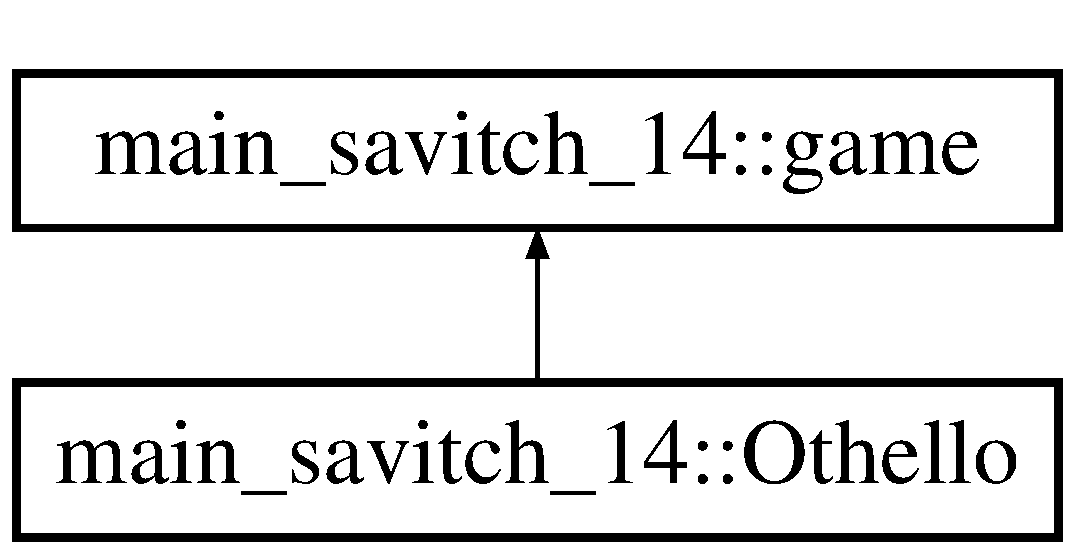
\includegraphics[height=2.000000cm]{classmain__savitch__14_1_1game}
\end{center}
\end{figure}
\subsection*{Public Types}
\begin{DoxyCompactItemize}
\item 
\mbox{\Hypertarget{classmain__savitch__14_1_1game_a4fe20fb287f809ae2b68e28e4ccba634}\label{classmain__savitch__14_1_1game_a4fe20fb287f809ae2b68e28e4ccba634}} 
enum {\bfseries who} \{ {\bfseries H\+U\+M\+AN}, 
{\bfseries N\+E\+U\+T\+R\+AL}, 
{\bfseries C\+O\+M\+P\+U\+T\+ER}
 \}
\end{DoxyCompactItemize}
\subsection*{Public Member Functions}
\begin{DoxyCompactItemize}
\item 
who \mbox{\hyperlink{classmain__savitch__14_1_1game_a4dbeaddb78059f7c5dcbf5cc4e026317}{play}} ()
\end{DoxyCompactItemize}
\subsection*{Protected Member Functions}
\begin{DoxyCompactItemize}
\item 
virtual void \mbox{\hyperlink{classmain__savitch__14_1_1game_ac58bfc07db8e604b07d2039b2cf7ab51}{display\+\_\+message}} (const std\+::string \&message) const
\item 
virtual std\+::string \mbox{\hyperlink{classmain__savitch__14_1_1game_a6504d401fcc8b138ae6342c2868c8a40}{get\+\_\+user\+\_\+move}} () const
\item 
\mbox{\Hypertarget{classmain__savitch__14_1_1game_a5c1ab8b36fb977bbe9fe387e793e4ee5}\label{classmain__savitch__14_1_1game_a5c1ab8b36fb977bbe9fe387e793e4ee5}} 
virtual who {\bfseries last\+\_\+mover} () const
\item 
\mbox{\Hypertarget{classmain__savitch__14_1_1game_a31dd5382cc6d64a6d58bcee55383cf1b}\label{classmain__savitch__14_1_1game_a31dd5382cc6d64a6d58bcee55383cf1b}} 
virtual int {\bfseries moves\+\_\+completed} () const
\item 
\mbox{\Hypertarget{classmain__savitch__14_1_1game_a4e68409618474d19742dd5f75f92f5c9}\label{classmain__savitch__14_1_1game_a4e68409618474d19742dd5f75f92f5c9}} 
virtual who {\bfseries next\+\_\+mover} () const
\item 
\mbox{\Hypertarget{classmain__savitch__14_1_1game_a98469e89e13c73a5ee70407a2164888c}\label{classmain__savitch__14_1_1game_a98469e89e13c73a5ee70407a2164888c}} 
virtual who {\bfseries opposite} (who player) const
\item 
\mbox{\Hypertarget{classmain__savitch__14_1_1game_a5954eccb6abf1ae900ad853ad2af99fa}\label{classmain__savitch__14_1_1game_a5954eccb6abf1ae900ad853ad2af99fa}} 
virtual void {\bfseries counting\+Pieces} ()=0
\item 
\mbox{\Hypertarget{classmain__savitch__14_1_1game_a98190a2bf784ce0f20533475754d136d}\label{classmain__savitch__14_1_1game_a98190a2bf784ce0f20533475754d136d}} 
virtual void {\bfseries whos\+Turn} ()=0
\item 
virtual who \mbox{\hyperlink{classmain__savitch__14_1_1game_a2f0d5338c12bd98d52fe2383ece5c45e}{winning}} () const
\item 
\mbox{\Hypertarget{classmain__savitch__14_1_1game_a20597d0caa907aea47b27fed8be3759b}\label{classmain__savitch__14_1_1game_a20597d0caa907aea47b27fed8be3759b}} 
virtual void {\bfseries make\+\_\+move} (const std\+::string \&move)
\item 
\mbox{\Hypertarget{classmain__savitch__14_1_1game_ad521a7d78e7c163a0bc28b709f0d45fd}\label{classmain__savitch__14_1_1game_ad521a7d78e7c163a0bc28b709f0d45fd}} 
virtual void {\bfseries restart} ()
\item 
\mbox{\Hypertarget{classmain__savitch__14_1_1game_a7b663057f59210dd52738facfc40d959}\label{classmain__savitch__14_1_1game_a7b663057f59210dd52738facfc40d959}} 
virtual \mbox{\hyperlink{classmain__savitch__14_1_1game}{game}} $\ast$ {\bfseries clone} () const =0
\item 
\mbox{\Hypertarget{classmain__savitch__14_1_1game_a2c0c049f5861026d0f639b5837889b7a}\label{classmain__savitch__14_1_1game_a2c0c049f5861026d0f639b5837889b7a}} 
virtual void {\bfseries compute\+\_\+moves} (std\+::queue$<$ std\+::string $>$ \&moves) const =0
\item 
virtual void \mbox{\hyperlink{classmain__savitch__14_1_1game_ac8205178922c49bab2865187e834b726}{display\+\_\+status}} () const =0
\begin{DoxyCompactList}\small\item\em This function displays the current state of the board to the user. \end{DoxyCompactList}\item 
\mbox{\Hypertarget{classmain__savitch__14_1_1game_a9b9c8c5e9aa57c9a430f20b87cb047aa}\label{classmain__savitch__14_1_1game_a9b9c8c5e9aa57c9a430f20b87cb047aa}} 
virtual int {\bfseries evaluate} () const =0
\item 
\mbox{\Hypertarget{classmain__savitch__14_1_1game_a49eed20648918b03fd3e2cf78987b3d1}\label{classmain__savitch__14_1_1game_a49eed20648918b03fd3e2cf78987b3d1}} 
virtual bool {\bfseries is\+\_\+game\+\_\+over} () const =0
\item 
\mbox{\Hypertarget{classmain__savitch__14_1_1game_ad38351422ca1ee3ae58440c1c6b36b30}\label{classmain__savitch__14_1_1game_ad38351422ca1ee3ae58440c1c6b36b30}} 
virtual bool {\bfseries is\+\_\+legal} (const std\+::string \&move) const =0
\end{DoxyCompactItemize}
\subsection*{Protected Attributes}
\begin{DoxyCompactItemize}
\item 
\mbox{\Hypertarget{classmain__savitch__14_1_1game_ac4c296f4370d8e5bb5ea74b638fb827d}\label{classmain__savitch__14_1_1game_ac4c296f4370d8e5bb5ea74b638fb827d}} 
int {\bfseries move\+\_\+number}
\end{DoxyCompactItemize}


\subsection{Member Function Documentation}
\mbox{\Hypertarget{classmain__savitch__14_1_1game_ac58bfc07db8e604b07d2039b2cf7ab51}\label{classmain__savitch__14_1_1game_ac58bfc07db8e604b07d2039b2cf7ab51}} 
\index{main\+\_\+savitch\+\_\+14\+::game@{main\+\_\+savitch\+\_\+14\+::game}!display\+\_\+message@{display\+\_\+message}}
\index{display\+\_\+message@{display\+\_\+message}!main\+\_\+savitch\+\_\+14\+::game@{main\+\_\+savitch\+\_\+14\+::game}}
\subsubsection{\texorpdfstring{display\+\_\+message()}{display\_message()}}
{\footnotesize\ttfamily void main\+\_\+savitch\+\_\+14\+::game\+::display\+\_\+message (\begin{DoxyParamCaption}\item[{const std\+::string \&}]{message }\end{DoxyParamCaption}) const\hspace{0.3cm}{\ttfamily [protected]}, {\ttfamily [virtual]}}

This function displays a message to the screen 
\begin{DoxyParams}{Parameters}
{\em message} & The message to be printed to the screen \\
\hline
\end{DoxyParams}
\begin{DoxyReturn}{Returns}
Nothing is returned 
\end{DoxyReturn}
\begin{DoxyAuthor}{Author}
Brock Ferrell Documentation by David Thompson 
\end{DoxyAuthor}
\mbox{\Hypertarget{classmain__savitch__14_1_1game_ac8205178922c49bab2865187e834b726}\label{classmain__savitch__14_1_1game_ac8205178922c49bab2865187e834b726}} 
\index{main\+\_\+savitch\+\_\+14\+::game@{main\+\_\+savitch\+\_\+14\+::game}!display\+\_\+status@{display\+\_\+status}}
\index{display\+\_\+status@{display\+\_\+status}!main\+\_\+savitch\+\_\+14\+::game@{main\+\_\+savitch\+\_\+14\+::game}}
\subsubsection{\texorpdfstring{display\+\_\+status()}{display\_status()}}
{\footnotesize\ttfamily virtual void main\+\_\+savitch\+\_\+14\+::game\+::display\+\_\+status (\begin{DoxyParamCaption}{ }\end{DoxyParamCaption}) const\hspace{0.3cm}{\ttfamily [protected]}, {\ttfamily [pure virtual]}}



This function displays the current state of the board to the user. 

Function name\+: display\+\_\+status Function Declaration \begin{DoxyAuthor}{Author}
Dr.\+Satvich(\+Documented by Mohamed Jallow) 
\end{DoxyAuthor}

\begin{DoxyParams}{Parameters}
{\em None} & \+:there are no parameters \\
\hline
\end{DoxyParams}
\begin{DoxyReturn}{Returns}
the function is void so it does not return a value. 
\end{DoxyReturn}


Implemented in \mbox{\hyperlink{classmain__savitch__14_1_1_othello_ab01a4f7aba130133221a11224905e8ce}{main\+\_\+savitch\+\_\+14\+::\+Othello}}.

\mbox{\Hypertarget{classmain__savitch__14_1_1game_a6504d401fcc8b138ae6342c2868c8a40}\label{classmain__savitch__14_1_1game_a6504d401fcc8b138ae6342c2868c8a40}} 
\index{main\+\_\+savitch\+\_\+14\+::game@{main\+\_\+savitch\+\_\+14\+::game}!get\+\_\+user\+\_\+move@{get\+\_\+user\+\_\+move}}
\index{get\+\_\+user\+\_\+move@{get\+\_\+user\+\_\+move}!main\+\_\+savitch\+\_\+14\+::game@{main\+\_\+savitch\+\_\+14\+::game}}
\subsubsection{\texorpdfstring{get\+\_\+user\+\_\+move()}{get\_user\_move()}}
{\footnotesize\ttfamily string main\+\_\+savitch\+\_\+14\+::game\+::get\+\_\+user\+\_\+move (\begin{DoxyParamCaption}{ }\end{DoxyParamCaption}) const\hspace{0.3cm}{\ttfamily [protected]}, {\ttfamily [virtual]}}

Function asks user for a move which the user then enters. If user cannot move then they enter \textquotesingle{}S\textquotesingle{} to the screen 
\begin{DoxyParams}{Parameters}
{\em No} & parameters passed to function \\
\hline
\end{DoxyParams}
\begin{DoxyReturn}{Returns}
A string is returned containing the users input of their move 
\end{DoxyReturn}
\begin{DoxyAuthor}{Author}
Brock Ferrell Documentation by David Thompson 
\end{DoxyAuthor}
\mbox{\Hypertarget{classmain__savitch__14_1_1game_a4dbeaddb78059f7c5dcbf5cc4e026317}\label{classmain__savitch__14_1_1game_a4dbeaddb78059f7c5dcbf5cc4e026317}} 
\index{main\+\_\+savitch\+\_\+14\+::game@{main\+\_\+savitch\+\_\+14\+::game}!play@{play}}
\index{play@{play}!main\+\_\+savitch\+\_\+14\+::game@{main\+\_\+savitch\+\_\+14\+::game}}
\subsubsection{\texorpdfstring{play()}{play()}}
{\footnotesize\ttfamily game\+::who main\+\_\+savitch\+\_\+14\+::game\+::play (\begin{DoxyParamCaption}{ }\end{DoxyParamCaption})}

This function returns whos turn it currently is in the game and weather or not the game has concluded 
\begin{DoxyParams}{Parameters}
{\em No} & parameters passed to function \\
\hline
\end{DoxyParams}
\begin{DoxyReturn}{Returns}
The winner of the game is returned 
\end{DoxyReturn}
\begin{DoxyAuthor}{Author}
Brock Ferrell Documentation by Daniel Ingram 
\end{DoxyAuthor}
\mbox{\Hypertarget{classmain__savitch__14_1_1game_a2f0d5338c12bd98d52fe2383ece5c45e}\label{classmain__savitch__14_1_1game_a2f0d5338c12bd98d52fe2383ece5c45e}} 
\index{main\+\_\+savitch\+\_\+14\+::game@{main\+\_\+savitch\+\_\+14\+::game}!winning@{winning}}
\index{winning@{winning}!main\+\_\+savitch\+\_\+14\+::game@{main\+\_\+savitch\+\_\+14\+::game}}
\subsubsection{\texorpdfstring{winning()}{winning()}}
{\footnotesize\ttfamily game\+::who main\+\_\+savitch\+\_\+14\+::game\+::winning (\begin{DoxyParamCaption}{ }\end{DoxyParamCaption}) const\hspace{0.3cm}{\ttfamily [protected]}, {\ttfamily [virtual]}}

Function determines whih player is currently winning the game 
\begin{DoxyParams}{Parameters}
{\em No} & parameters passed to function \\
\hline
\end{DoxyParams}
\begin{DoxyReturn}{Returns}
Function returns enum who which is either Human, Computer, or neutral depending on who is winning 
\end{DoxyReturn}
\begin{DoxyAuthor}{Author}
Brock Ferrell Documentation by David Thompson 
\end{DoxyAuthor}


Reimplemented in \mbox{\hyperlink{classmain__savitch__14_1_1_othello_a4ea78b18eea66c944c0a9356349e0fd4}{main\+\_\+savitch\+\_\+14\+::\+Othello}}.



The documentation for this class was generated from the following files\+:\begin{DoxyCompactItemize}
\item 
game.\+h\item 
\mbox{\hyperlink{game_8cc}{game.\+cc}}\end{DoxyCompactItemize}

\hypertarget{classmain__savitch__14_1_1_othello}{}\section{main\+\_\+savitch\+\_\+14\+:\+:Othello Class Reference}
\label{classmain__savitch__14_1_1_othello}\index{main\+\_\+savitch\+\_\+14\+::\+Othello@{main\+\_\+savitch\+\_\+14\+::\+Othello}}
Inheritance diagram for main\+\_\+savitch\+\_\+14\+:\+:Othello\+:\begin{figure}[H]
\begin{center}
\leavevmode
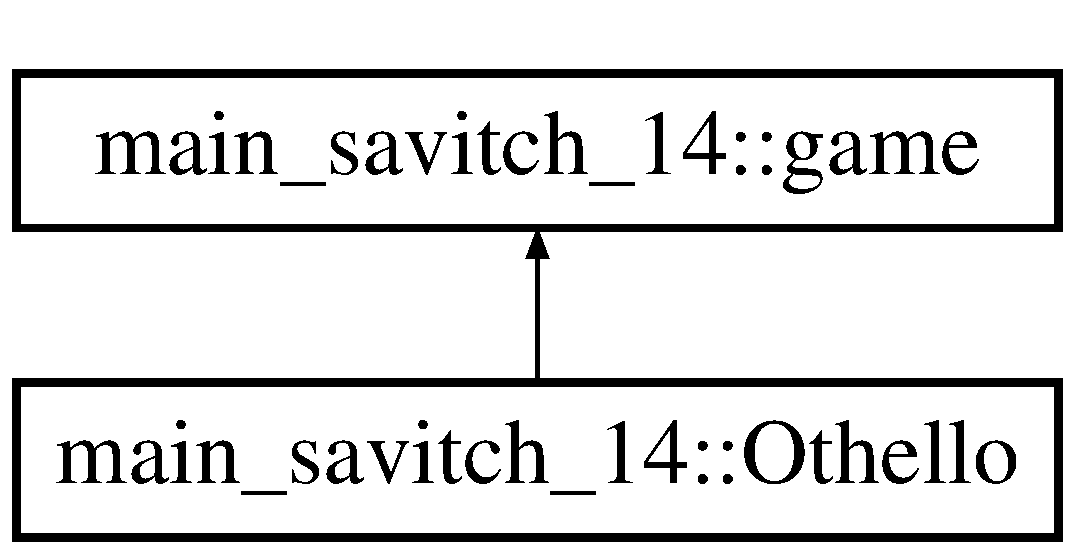
\includegraphics[height=2.000000cm]{classmain__savitch__14_1_1_othello}
\end{center}
\end{figure}
\subsection*{Public Member Functions}
\begin{DoxyCompactItemize}
\item 
void \mbox{\hyperlink{classmain__savitch__14_1_1_othello_ab01a4f7aba130133221a11224905e8ce}{display\+\_\+status}} () const
\begin{DoxyCompactList}\small\item\em This function displays the current state of the board to the user. \end{DoxyCompactList}\item 
\mbox{\Hypertarget{classmain__savitch__14_1_1_othello_a57ae44590de8d683592f186ed6bd25b0}\label{classmain__savitch__14_1_1_othello_a57ae44590de8d683592f186ed6bd25b0}} 
int {\bfseries evaluate} () const
\item 
\mbox{\Hypertarget{classmain__savitch__14_1_1_othello_a540c8b0030e429e0ac30f07e9e8868ec}\label{classmain__savitch__14_1_1_othello_a540c8b0030e429e0ac30f07e9e8868ec}} 
bool {\bfseries is\+\_\+game\+\_\+over} () const
\item 
\mbox{\Hypertarget{classmain__savitch__14_1_1_othello_a74ac0d4e6399167037dfc708efdb9033}\label{classmain__savitch__14_1_1_othello_a74ac0d4e6399167037dfc708efdb9033}} 
bool {\bfseries is\+\_\+legal} (const string \&move) const
\item 
\mbox{\Hypertarget{classmain__savitch__14_1_1_othello_a1066b280efa5cb41039585669282fe06}\label{classmain__savitch__14_1_1_othello_a1066b280efa5cb41039585669282fe06}} 
void {\bfseries make\+\_\+move} (const string \&move)
\item 
void \mbox{\hyperlink{classmain__savitch__14_1_1_othello_abf872b8074bfa4c04119317dc3b39af2}{restart}} ()
\item 
\mbox{\Hypertarget{classmain__savitch__14_1_1_othello_a3177234195a490eef52343d957e64b5d}\label{classmain__savitch__14_1_1_othello_a3177234195a490eef52343d957e64b5d}} 
void {\bfseries make\+\_\+skips} ()
\item 
\mbox{\Hypertarget{classmain__savitch__14_1_1_othello_a19f49edfbe82b84922877e00bc854ed8}\label{classmain__savitch__14_1_1_othello_a19f49edfbe82b84922877e00bc854ed8}} 
void {\bfseries counting\+Pieces} ()
\item 
\mbox{\Hypertarget{classmain__savitch__14_1_1_othello_a21440dbb4511812a76c578a5f546710b}\label{classmain__savitch__14_1_1_othello_a21440dbb4511812a76c578a5f546710b}} 
void {\bfseries whos\+Turn} ()
\item 
\mbox{\Hypertarget{classmain__savitch__14_1_1_othello_a7a5f8495f1a61f6e7b3968e919013c18}\label{classmain__savitch__14_1_1_othello_a7a5f8495f1a61f6e7b3968e919013c18}} 
\mbox{\hyperlink{classmain__savitch__14_1_1game}{game}} $\ast$ {\bfseries clone} () const
\item 
\mbox{\Hypertarget{classmain__savitch__14_1_1_othello_a921d4ffa277b0250f187f20b9598ebb1}\label{classmain__savitch__14_1_1_othello_a921d4ffa277b0250f187f20b9598ebb1}} 
void {\bfseries compute\+\_\+moves} (std\+::queue$<$ std\+::string $>$ \&moves) const
\item 
who \mbox{\hyperlink{classmain__savitch__14_1_1_othello_a4ea78b18eea66c944c0a9356349e0fd4}{winning}} () const
\end{DoxyCompactItemize}
\subsection*{Protected Attributes}
\begin{DoxyCompactItemize}
\item 
\mbox{\Hypertarget{classmain__savitch__14_1_1_othello_a2eed818925f68d5678b78107a3298138}\label{classmain__savitch__14_1_1_othello_a2eed818925f68d5678b78107a3298138}} 
int {\bfseries black}
\item 
\mbox{\Hypertarget{classmain__savitch__14_1_1_othello_a7d5f59b1e581ed7a8145debeecf4f310}\label{classmain__savitch__14_1_1_othello_a7d5f59b1e581ed7a8145debeecf4f310}} 
int {\bfseries white}
\item 
\mbox{\Hypertarget{classmain__savitch__14_1_1_othello_a85d4ce17512d8dbf85a313a27eea0644}\label{classmain__savitch__14_1_1_othello_a85d4ce17512d8dbf85a313a27eea0644}} 
int {\bfseries skips}
\item 
\mbox{\Hypertarget{classmain__savitch__14_1_1_othello_a15045e3e94c34afe08240885e230d502}\label{classmain__savitch__14_1_1_othello_a15045e3e94c34afe08240885e230d502}} 
int {\bfseries open\+Spots}
\item 
\mbox{\Hypertarget{classmain__savitch__14_1_1_othello_a98fbc46241d2f5e05ccb4b66f11535bf}\label{classmain__savitch__14_1_1_othello_a98fbc46241d2f5e05ccb4b66f11535bf}} 
int {\bfseries b}
\item 
\mbox{\Hypertarget{classmain__savitch__14_1_1_othello_a1b11c5fe33e30a94ed39e8cb55caf37e}\label{classmain__savitch__14_1_1_othello_a1b11c5fe33e30a94ed39e8cb55caf37e}} 
int {\bfseries w}
\end{DoxyCompactItemize}
\subsection*{Additional Inherited Members}


\subsection{Member Function Documentation}
\mbox{\Hypertarget{classmain__savitch__14_1_1_othello_ab01a4f7aba130133221a11224905e8ce}\label{classmain__savitch__14_1_1_othello_ab01a4f7aba130133221a11224905e8ce}} 
\index{main\+\_\+savitch\+\_\+14\+::\+Othello@{main\+\_\+savitch\+\_\+14\+::\+Othello}!display\+\_\+status@{display\+\_\+status}}
\index{display\+\_\+status@{display\+\_\+status}!main\+\_\+savitch\+\_\+14\+::\+Othello@{main\+\_\+savitch\+\_\+14\+::\+Othello}}
\subsubsection{\texorpdfstring{display\+\_\+status()}{display\_status()}}
{\footnotesize\ttfamily void main\+\_\+savitch\+\_\+14\+::\+Othello\+::display\+\_\+status (\begin{DoxyParamCaption}{ }\end{DoxyParamCaption}) const\hspace{0.3cm}{\ttfamily [virtual]}}



This function displays the current state of the board to the user. 

Function name\+: display\+\_\+status \begin{DoxyAuthor}{Author}
Brock Ferrell(\+Documented by Mohamed Jallow) Function Declaration 
\end{DoxyAuthor}

\begin{DoxyParams}{Parameters}
{\em None} & \+:there are no parameters \\
\hline
\end{DoxyParams}
\begin{DoxyReturn}{Returns}
the function is void so it does not return a value.
\end{DoxyReturn}
Function name\+: display\+\_\+status \begin{DoxyAuthor}{Author}
Brock Ferrell(\+Documented by Mohamed Jallow) Function definition 
\end{DoxyAuthor}

\begin{DoxyParams}{Parameters}
{\em None} & \+:there are no parameters \\
\hline
\end{DoxyParams}
\begin{DoxyReturn}{Returns}
the function is void so it does not return a value. 
\end{DoxyReturn}


Implements \mbox{\hyperlink{classmain__savitch__14_1_1game_ac8205178922c49bab2865187e834b726}{main\+\_\+savitch\+\_\+14\+::game}}.

\mbox{\Hypertarget{classmain__savitch__14_1_1_othello_abf872b8074bfa4c04119317dc3b39af2}\label{classmain__savitch__14_1_1_othello_abf872b8074bfa4c04119317dc3b39af2}} 
\index{main\+\_\+savitch\+\_\+14\+::\+Othello@{main\+\_\+savitch\+\_\+14\+::\+Othello}!restart@{restart}}
\index{restart@{restart}!main\+\_\+savitch\+\_\+14\+::\+Othello@{main\+\_\+savitch\+\_\+14\+::\+Othello}}
\subsubsection{\texorpdfstring{restart()}{restart()}}
{\footnotesize\ttfamily void main\+\_\+savitch\+\_\+14\+::\+Othello\+::restart (\begin{DoxyParamCaption}{ }\end{DoxyParamCaption})\hspace{0.3cm}{\ttfamily [virtual]}}

Function name\+: display\+\_\+status \begin{DoxyAuthor}{Author}
Brock Ferrell(\+Documented by Carter Hickman)
\end{DoxyAuthor}
This function restarts the graphical game board back to normal for start of a new game. 
\begin{DoxyParams}{Parameters}
{\em None} & \+:there are no parameters \\
\hline
\end{DoxyParams}
\begin{DoxyReturn}{Returns}
the function is void so it does not return a value.
\end{DoxyReturn}


Reimplemented from \mbox{\hyperlink{classmain__savitch__14_1_1game}{main\+\_\+savitch\+\_\+14\+::game}}.

\mbox{\Hypertarget{classmain__savitch__14_1_1_othello_a4ea78b18eea66c944c0a9356349e0fd4}\label{classmain__savitch__14_1_1_othello_a4ea78b18eea66c944c0a9356349e0fd4}} 
\index{main\+\_\+savitch\+\_\+14\+::\+Othello@{main\+\_\+savitch\+\_\+14\+::\+Othello}!winning@{winning}}
\index{winning@{winning}!main\+\_\+savitch\+\_\+14\+::\+Othello@{main\+\_\+savitch\+\_\+14\+::\+Othello}}
\subsubsection{\texorpdfstring{winning()}{winning()}}
{\footnotesize\ttfamily game\+::who main\+\_\+savitch\+\_\+14\+::\+Othello\+::winning (\begin{DoxyParamCaption}{ }\end{DoxyParamCaption}) const\hspace{0.3cm}{\ttfamily [virtual]}}

Function determines whih player is currently winning the game 
\begin{DoxyParams}{Parameters}
{\em No} & parameters passed to function \\
\hline
\end{DoxyParams}
\begin{DoxyReturn}{Returns}
Function returns enum who which is either Human, Computer, or neutral depending on who is winning 
\end{DoxyReturn}
\begin{DoxyAuthor}{Author}
Brock Ferrell Documentation by David Thompson 
\end{DoxyAuthor}


Reimplemented from \mbox{\hyperlink{classmain__savitch__14_1_1game_a2f0d5338c12bd98d52fe2383ece5c45e}{main\+\_\+savitch\+\_\+14\+::game}}.



The documentation for this class was generated from the following files\+:\begin{DoxyCompactItemize}
\item 
\mbox{\hyperlink{othello_8h}{othello.\+h}}\item 
\mbox{\hyperlink{othello_8cc}{othello.\+cc}}\end{DoxyCompactItemize}

\hypertarget{classpiece}{}\section{piece Class Reference}
\label{classpiece}\index{piece@{piece}}
\subsection*{Public Member Functions}
\begin{DoxyCompactItemize}
\item 
\mbox{\Hypertarget{classpiece_ab898c5827a5859e4cddc9d61a814a873}\label{classpiece_ab898c5827a5859e4cddc9d61a814a873}} 
void {\bfseries flip} ()
\item 
bool \mbox{\hyperlink{classpiece_aa1eda7729e0f3383a813fc6ccc4e7e3c}{is\+\_\+blank}} () const
\begin{DoxyCompactList}\small\item\em This function returns the boolean value for the conditional \char`\"{}the\+Color == blank\char`\"{}. \end{DoxyCompactList}\item 
\mbox{\Hypertarget{classpiece_a103dccd216cb495d1c42b2465778be53}\label{classpiece_a103dccd216cb495d1c42b2465778be53}} 
bool {\bfseries is\+\_\+black} () const
\item 
\mbox{\Hypertarget{classpiece_ae9dde29687fcb2b7badc6cb5395a13f2}\label{classpiece_ae9dde29687fcb2b7badc6cb5395a13f2}} 
bool {\bfseries is\+\_\+white} () const
\item 
\mbox{\Hypertarget{classpiece_a31480899f2a591fdb22d97933303e19d}\label{classpiece_a31480899f2a591fdb22d97933303e19d}} 
void {\bfseries set\+\_\+white} ()
\item 
\mbox{\Hypertarget{classpiece_a273d63d07b6ea973b2fc4f7e1b56ea10}\label{classpiece_a273d63d07b6ea973b2fc4f7e1b56ea10}} 
void {\bfseries set\+\_\+black} ()
\end{DoxyCompactItemize}


\subsection{Member Function Documentation}
\mbox{\Hypertarget{classpiece_aa1eda7729e0f3383a813fc6ccc4e7e3c}\label{classpiece_aa1eda7729e0f3383a813fc6ccc4e7e3c}} 
\index{piece@{piece}!is\+\_\+blank@{is\+\_\+blank}}
\index{is\+\_\+blank@{is\+\_\+blank}!piece@{piece}}
\subsubsection{\texorpdfstring{is\+\_\+blank()}{is\_blank()}}
{\footnotesize\ttfamily bool piece\+::is\+\_\+blank (\begin{DoxyParamCaption}{ }\end{DoxyParamCaption}) const\hspace{0.3cm}{\ttfamily [inline]}}



This function returns the boolean value for the conditional \char`\"{}the\+Color == blank\char`\"{}. 

Function name\+: is\+\_\+blank \begin{DoxyAuthor}{Author}
Brock Ferrell(\+Documented by Mohamed Jallow) Function Declaration 
\end{DoxyAuthor}

\begin{DoxyParams}{Parameters}
{\em None} & \+:there are no parameters \\
\hline
\end{DoxyParams}
\begin{DoxyReturn}{Returns}
the function returns true or false depeding on what is stored in the the\+Color variable. 
\end{DoxyReturn}


The documentation for this class was generated from the following file\+:\begin{DoxyCompactItemize}
\item 
\mbox{\hyperlink{piece_8h}{piece.\+h}}\end{DoxyCompactItemize}

\chapter{File Documentation}
\hypertarget{game_8cc}{}\section{game.\+cc File Reference}
\label{game_8cc}\index{game.\+cc@{game.\+cc}}


Initiates start of game and checks for end of game/restart. Calls for humans or computer to make move and will move for computer. Looks for best moves with function look ahead. The majority of the functionality of the game is here.  


{\ttfamily \#include $<$cassert$>$}\newline
{\ttfamily \#include $<$climits$>$}\newline
{\ttfamily \#include $<$iostream$>$}\newline
{\ttfamily \#include $<$queue$>$}\newline
{\ttfamily \#include $<$string$>$}\newline
{\ttfamily \#include \char`\"{}game.\+h\char`\"{}}\newline


\subsection{Detailed Description}
Initiates start of game and checks for end of game/restart. Calls for humans or computer to make move and will move for computer. Looks for best moves with function look ahead. The majority of the functionality of the game is here. 

header file for \mbox{\hyperlink{game_8cc}{game.\+cc}}

\begin{DoxyAuthor}{Author}
Brock Ferrell(documented by Carter Hickman) 
\end{DoxyAuthor}

\hypertarget{main_8cc}{}\section{main.\+cc File Reference}
\label{main_8cc}\index{main.\+cc@{main.\+cc}}


Start, restart called here. No functionality, only calls for came to play or restart.  


{\ttfamily \#include \char`\"{}game.\+h\char`\"{}}\newline
{\ttfamily \#include \char`\"{}othello.\+h\char`\"{}}\newline
\subsection*{Functions}
\begin{DoxyCompactItemize}
\item 
int \mbox{\hyperlink{main_8cc_ae66f6b31b5ad750f1fe042a706a4e3d4}{main}} ()
\begin{DoxyCompactList}\small\item\em This function creates an Othello object named the\+Game, runs the restart function, then runs the play function. \end{DoxyCompactList}\end{DoxyCompactItemize}


\subsection{Detailed Description}
Start, restart called here. No functionality, only calls for came to play or restart. 

\begin{DoxyAuthor}{Author}
Brock Ferrell (documented by Carter Hickman) 
\end{DoxyAuthor}


\subsection{Function Documentation}
\mbox{\Hypertarget{main_8cc_ae66f6b31b5ad750f1fe042a706a4e3d4}\label{main_8cc_ae66f6b31b5ad750f1fe042a706a4e3d4}} 
\index{main.\+cc@{main.\+cc}!main@{main}}
\index{main@{main}!main.\+cc@{main.\+cc}}
\subsubsection{\texorpdfstring{main()}{main()}}
{\footnotesize\ttfamily int main (\begin{DoxyParamCaption}{ }\end{DoxyParamCaption})}



This function creates an Othello object named the\+Game, runs the restart function, then runs the play function. 

Function name\+: \mbox{\hyperlink{main_8cc_ae66f6b31b5ad750f1fe042a706a4e3d4}{main()}} \begin{DoxyAuthor}{Author}
Brock Ferrell(\+Documented by Mohamed Jallow) 
\end{DoxyAuthor}

\begin{DoxyParams}{Parameters}
{\em None} & \+:there are no parameters \\
\hline
\end{DoxyParams}
\begin{DoxyReturn}{Returns}
the function returns the value 0. 
\end{DoxyReturn}

\hypertarget{othello_8cc}{}\section{othello.\+cc File Reference}
\label{othello_8cc}\index{othello.\+cc@{othello.\+cc}}


This displays the graphics for the game board, checks if game is over, checks for legal moves, executes moves, computes new moves, restarts game, skips turn, and checks whose turn it is.  


{\ttfamily \#include \char`\"{}othello.\+h\char`\"{}}\newline


\subsection{Detailed Description}
This displays the graphics for the game board, checks if game is over, checks for legal moves, executes moves, computes new moves, restarts game, skips turn, and checks whose turn it is. 

\begin{DoxyAuthor}{Author}
Brock Ferrell (documented by Carter Hickman) 
\end{DoxyAuthor}

\hypertarget{othello_8h}{}\section{othello.\+h File Reference}
\label{othello_8h}\index{othello.\+h@{othello.\+h}}


.h file for \mbox{\hyperlink{othello_8cc}{othello.\+cc}}. Private variables and functions declared here.  


{\ttfamily \#include \char`\"{}game.\+h\char`\"{}}\newline
{\ttfamily \#include \char`\"{}piece.\+h\char`\"{}}\newline
{\ttfamily \#include \char`\"{}colors.\+h\char`\"{}}\newline
{\ttfamily \#include $<$iostream$>$}\newline
\subsection*{Classes}
\begin{DoxyCompactItemize}
\item 
class \mbox{\hyperlink{classmain__savitch__14_1_1_othello}{main\+\_\+savitch\+\_\+14\+::\+Othello}}
\end{DoxyCompactItemize}


\subsection{Detailed Description}
.h file for \mbox{\hyperlink{othello_8cc}{othello.\+cc}}. Private variables and functions declared here. 

\begin{DoxyAuthor}{Author}
Brock Ferrell(documented by Carter Hickman) 
\end{DoxyAuthor}

\hypertarget{piece_8h}{}\section{piece.\+h File Reference}
\label{piece_8h}\index{piece.\+h@{piece.\+h}}


Defines each space on board as a piece. Sets pieces to white or black depending.  


\subsection*{Classes}
\begin{DoxyCompactItemize}
\item 
class \mbox{\hyperlink{classpiece}{piece}}
\end{DoxyCompactItemize}
\subsection*{Enumerations}
\begin{DoxyCompactItemize}
\item 
\mbox{\Hypertarget{piece_8h_a37dbdc30935031c05304482e1be89d8f}\label{piece_8h_a37dbdc30935031c05304482e1be89d8f}} 
enum {\bfseries color} \{ {\bfseries black}, 
{\bfseries white}, 
{\bfseries blank}
 \}
\end{DoxyCompactItemize}


\subsection{Detailed Description}
Defines each space on board as a piece. Sets pieces to white or black depending. 

\begin{DoxyAuthor}{Author}
Brock Ferrell (documented by Carter Hickman) 
\end{DoxyAuthor}

%--- End generated contents ---

% Index
\backmatter
\newpage
\phantomsection
\clearemptydoublepage
\addcontentsline{toc}{chapter}{Index}
\printindex

\end{document}
